% !TeX encoding = UTF-8
%



\clearpage



% Fehlende Bestandteile.
	
\subsection*{Testsysteme}

Die Hardware, welche wir beim Testen in den Extremtests verwendet haben.\\

~\\



\phantomsection
\label{Anhang:Testsysteme:Notebook}



\begin{figure}[ht!]

	\centering
	\label{Anhang:Medien:Acer_Travelmate5742G_CPU}
	
	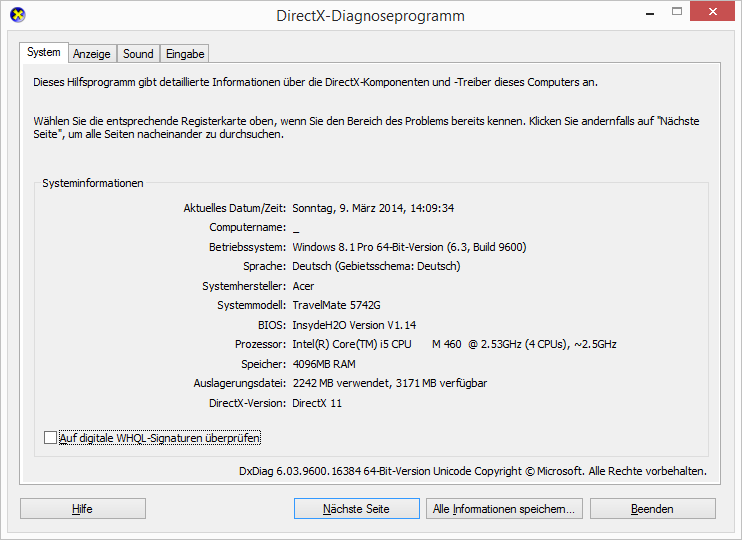
\includegraphics[width=0.7\textwidth]{\Media/Acer_Travelmate5742G_CPU.png}
	
	\caption{Systemeigenschaften - CPU (Notebook).}

\end{figure}

\begin{figure}[ht!]

	\centering
	\label{Anhang:Medien:Acer_Travelmate5742G_GPU}
	
	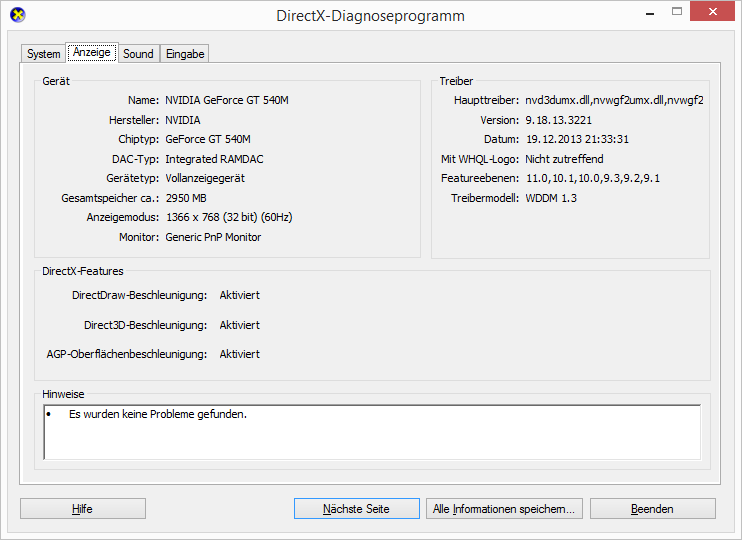
\includegraphics[width=0.7\textwidth]{\Media/Acer_Travelmate5742G_GPU.png}
	
	\caption{Systemeigenschaften - GPU (Notebook).}

\end{figure}


~\\~\mousecursor~\hyperref[Abschnitt:Tests:Protokoll:Extrem:Knoten_Erzeugen:Notebook]{Zurück zu den Extremtests unter Abschnitt \ref{Abschnitt:Tests:Protokoll}, ab S. \pageref{Abschnitt:Tests:Protokoll:Extrem:Knoten_Erzeugen:Notebook}.}


\clearpage



\phantomsection
\label{Anhang:Testsysteme:Desktop}



\begin{figure}[ht!]

	\centering
	\label{Anhang:Medien:Asus_CPU}
	
	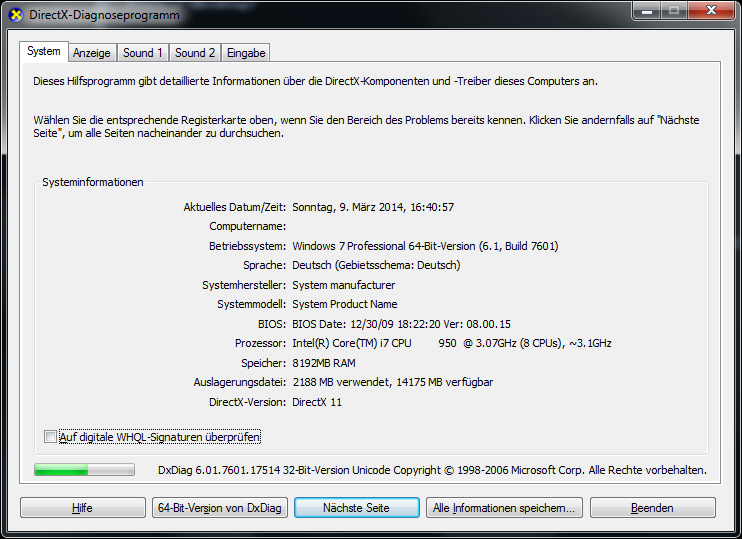
\includegraphics[width=0.75\textwidth]{\Media/Asus_CPU.png}
	
	\caption{Systemeigenschaften - CPU (Desktop).}

\end{figure}

\begin{figure}[ht!]

	\centering
	\label{Anhang:Medien:Asus_GPU}
	
	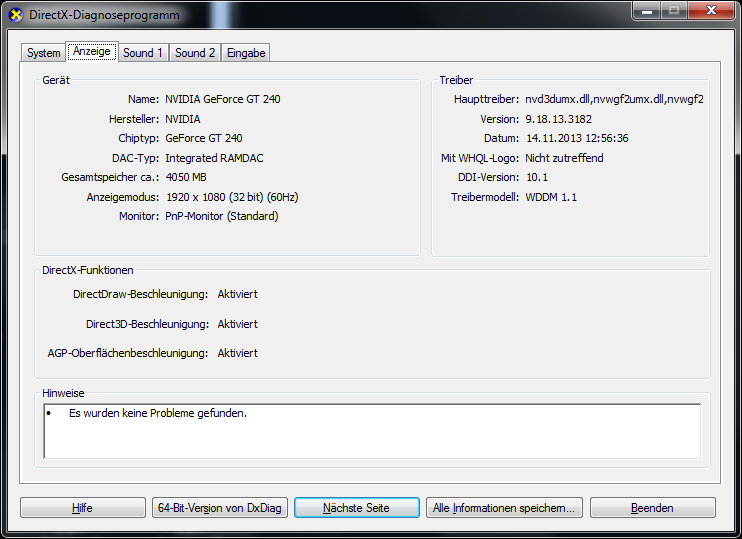
\includegraphics[width=0.75\textwidth]{\Media/Asus_GPU.png}
	
	\caption{Systemeigenschaften - GPU (Desktop).}

\end{figure}

~\\~\mousecursor~\hyperref[Abschnitt:Tests:Protokoll:Extrem:Knoten_Erzeugen:Desktop]{Zurück zu den Extremtests unter Abschnitt \ref{Abschnitt:Tests:Protokoll}, ab S. \pageref{Abschnitt:Tests:Protokoll:Extrem:Knoten_Erzeugen:Desktop}.}


